\chapter{Neutrinos in cosmic plasma}\label{Neutrino}
Neutrinos are fundamental particles and play an important role in the evolution of the Universe. In the early Universe the neutrinos are kept in equilibrium with cosmic plasma via the weak interaction. The neutrino-matter interactions play a crucial role in  understanding of neutrinos evolution in the early Universe (such as the neutrino freezeout) and the later Universe (the property of today's neutrino background). In this chapter, I will examine the neutrino coherent and incoherent scattering with matter and their application in cosmology. The investigation of the relation between the effective number of neutrinos $N^{\mathrm{eff}}_\nu$ and lepton asymmetry $L$ after neutrino freezeout and its impact on Universe expansion is also discussed in this chapter. 

%{Introduction\daggerfootnote{This chapter has been published previously as \citet{Gottbrath1999}.}}

%~~~~~~~~~~~~~~~~~~~~~~~~~~~~~~~~~~~~~~~~~~~~~~~~~

%\section{Neutrino in particle physics}
%From the standard neutrino oscillation theory, the neutrino flavor eigenstate $\nu^{\alpha}$ can be described as a superposition of mass eigenstates $\nu_{k}$ as follow:
%\begin{align}\label{NuFlavors}
%	\nu_{\alpha}=\sum_k^nU^\ast_{\alpha k}\nu_{k}, \qquad\alpha=e,\mu,\tau,\qquad k=1,2,3,\dots,n
%\end{align}
%where $U$ is the the Pontecorvo-Maki-Nakagawa-Sakata (PMNS) mixing matrix~[\cite{King:2013eh,FernandezMartinez:2016lgt}] which are both in general complex and unitary. Evaluating freely propagating plane waves in the relativistic limit yields the vacuum oscillation probability between flavors $\nu_\alpha$ and $\nu_\beta$ written as~[\cite{ParticleDataGroup:2022pth}]
%\begin{align}\label{NuOscillation}
%  P_{\alpha\rightarrow\beta}
% =&\delta_{\alpha\beta}-4\sum_{i<j}^n \mathrm{Re}\left[U_{\alpha i}U^\ast_{\beta i}U^\ast_{\alpha j}U_{\beta j}\right]\sin^2\!\!\left(\frac{\Delta m^2_{ij}L}{4E}\right)\notag\\
% &+2\sum_{i<j}^n \mathrm{Im}\left[U_{\alpha i}U^\ast_{\beta i}U^\ast_{\alpha j}U_{\beta j}\right]\sin\!\!\left(\frac{\Delta m^2_{ij}L}{2E}\right)
% ,\qquad\Delta m^2_{ij}\equiv{m^2_i-m^2_j}
%\end{align}
%where $L$ is the distance traveled by the neutrino between production and detection. The square mass difference $\Delta m^2_{ij}$ has been experimentally measured, from the neutrino oscillation experiment~[\cite{ParticleDataGroup:2022pth}]:
%\begin{align}
%&\Delta{m}_{21}^2=7.39^{+0.21}_{-0.20}\times10^{-5}\,\mathrm{eV}^2,\\
%&\Delta{m}_{32}^2=2.45^{+0.03}_{-0.03}\times10^{-3}\,\mathrm{eV}^2.
%\end{align}
%and neutrino mass eigenvalue can be ordered in the normal mass hierarchy ($m_1\ll m_2<m_3$) or inverted mass hierarchy ($m_3\ll m_1<m_2$). All three mass states remained relativistic until the temperature dropped below their rest mass. These results allow for the possibility that one mass eigenstate or two mass eigenstates of neutrinos may become non-relativistic today. 

%In this chapter, we discuss the neutrino interaction with matter coherent/incoherent scattering, an overview of neutrino freezeout and effective number of neutrino in early Universe.


%~~~~~~~~~~~~~~~~~~~~~~~~~~~~~~~~~~~~~~~~~~~~~~~~~

\section{Matrix element for neutrino coherent/ incoherent scattering}
 According to the standard model, neutrinos interact with other particles via the Charged-Current(CC) and Neutral-Current(NC) interactions. Their Lagrangian can be written as~[\cite{Giunti:2007ry}]
\begin{align}
&\mathcal{L}^{CC}=\frac{g}{2\sqrt{2}}\left(j^\mu_W\,W_\mu+{j^\mu_W}^\dagger\,W^\dagger_\mu\right),\qquad\mathcal{L}^{NC}=-\frac{g}{2\cos{\theta_w}}\,j^\mu_Z\,Z_\mu,
\end{align}
where $g=e\sin\theta_w$, $W^\mu$ and $Z^\mu$ are W and Z boson gauge fields, and $j^\mu_W$ and $j^\mu_Z$ are the charged-current and neutral-current separately. In the limit of energies lower than the $W(m_w=80\,\mathrm{GeV})$ and $Z(m_z=91\,\mathrm{GeV})$ gauge bosons, the effective Lagrangians are given by
\begin{align}\label{L_low}
\mathcal{L}^{CC}_{eff}=-\frac{G_F}{\sqrt{2}}\,j^\dagger_{W\,\mu}\,j^\mu_W,\qquad
\mathcal{L}^{NC}_{eff}=-\frac{G_F}{\sqrt{2}}\,j^\dagger_{Z\,\mu}\,j^\mu_Z,\qquad \frac{G_F}{\sqrt{2}}=\frac{g^2}{8m^2_W},
\end{align}
where $G_F=1.1664\times10^{-5}\,\mathrm{GeV}^{-2}$ is the Fermi constant, which is one of the important parameters that determine the strength of the weak interaction rate. When neutrinos interact with matter, based on the neutrino's wavelength, they can undergo two types of scattering processes: coherent scattering and incoherent scattering with the particles in the medium. 

With coherent scattering, neutrinos interact with the entire  composite system rather than individual particles within the system. The coherent scattering is particularly relevant for low-energy neutrinos when the wavelength of neutrino is much larger than the size of system. In $1978$, Lincoln Wolfenstein pointed out that the coherent forward scattering of neutrinos off matter could be very important in studying the behavior of neutrino flavor oscillation in a dense medium~[\cite{PhysRevD.17.2369}]. The fact that neutrinos propagating in matter may interact with the background particles can be described by the picture of free neutrinos traveling in an effective potential.

For incoherent scattering, neutrinos interact with particles in the medium individually. Incoherent scattering is typically more prominent for high-energy neutrinos, where the wavelength of neutrino is smaller compared to the spacing between particles. Study of incoherent scattering of high-energy neutrinos is important for understanding the physics in various astrophysical systems (e.g. supernova, stellar formation) and the evolution of the early Universe.

In this section, we discuss the coherent scattering between long wavelength neutrinos and atoms, and study the effective potential for neutrino coherent interaction. Then we present the matrix elements that describe the incoherent interaction between high energy neutrinos and other fundamental particles in the early Universe. Understanding these matrix elements is crucial for comprehending the process of neutrino freeze-out in the early Universe.

%~~~~~~~~~~~~~~~~~~~~~~~~~~~~~~~~~~~~~~~~~~~~~~~~~~~~~~~~~~~~~~~~~~~~~~~

\subsection{Long wavelength limit of neutrino-atom coherent scattering}\label{LongWavelength}
According to the standard cosmological model, the Universe today is filled with the cosmic neutrinos with temperature $T_{\nu}^0=1.9 \,\mathrm{K}=1.7\times10^{-4}\,\mathrm{eV}$.
The average momentum of present-day relic neutrinos is given by $\langle p_\nu^0\rangle\approx3.15\,T_\nu^0$ and the typical wavelength $\lambda_\nu^0={2\pi}/{\langle p_\nu^0\rangle}\approx2.3\times10^5\,\mathrm{\AA}$, which is much larger than the radius at the atomic scale, such as the Bohr radius $R_{\mathrm{atom}}=0.529\,\mathrm{\AA}$. In this case we have the long wavelength condition $\lambda_\nu\gg\,R_{\mathrm{atom}}$ for cosmic neutrino background today.  

Under the condition $\lambda_\nu\gg\,R_{\mathrm{atom}}$, when the neutrino is scattering off an atom, the interaction can be coherent scattering [\cite{PhysRevD.38.32,PhysRevD.21.663,Papavassiliou:2005cs}]. According to the principles of quantum mechanics, with neutrino scattering it is impossible to identify which scatters the neutrino interacts with and thus it is necessary to sum over all possible contributions. In such circumstances, it is appropriate to view the scattering reaction as taking place on the atom as a whole, i.e.,
\begin{align}
\nu+\mathrm{Atom}\longrightarrow\nu+\mathrm{Atom}.
\end{align}

Considering a neutrino elastic scattering off an atom which is composed of $Z$ protons, $N$ neutrons and $Z$ electrons. For the elastic neutrino atom scattering, the low-energy neutrinos scatter off both atomic electrons and nucleus. For nucleus parts, we consider that the neutrinos interact via the $Z^0$ boson with a nucleus as
\begin{align}
\nu+A^{Z}_N\longrightarrow\nu+A^{Z}_N.
\end{align}
In this process a neutrino of any flavor scatters off a nucleus with the same strength. Therefore, the scattering will be insensitive to neutrino flavor. On the other hand, the neutrons can also interact via the $W^\pm$ with nucleus as 
\begin{align}
\nu_l+A^{Z}_N\longrightarrow\,l^-+A^{{Z}+1}_N,
\end{align}
which is a quasi-elastic process for neutrino scattering with the nucleus; we have $A^{Z_e}_N\rightarrow\,A^{{Z_e}+1}_N$. Since this process will change the nucleus state into an excited one, we will not consider its effect here. For detail discussion pf quasi-elastic scattering see ~[\cite{SajjadAthar:2022pjt}].

For atomic electrons, the neutrinos can interact via the $Z^0$ and $W^\pm$ bosons with electrons for different flavors, we have
\begin{align}
&\nu_e+e^-\longrightarrow\nu_e+e^-\,\,\,(\mathrm{Z^0,\,W^\pm\,exchange}),\\
&\nu_{\mu,\tau}+e^-\longrightarrow\nu_{\mu,\tau}+e^-\,\,\,(\mathrm{Z^0\,exchange}).
\end{align}
Because of the fact that the coupling of $\nu_e$ to electrons is quite different from that of $\nu_{\mu,\tau}$, one may expect large differences in the behavior of $\nu_e$ scattering compared to the other neutrino types.


%~~~~~~~~~~~~~~~~~~~~~~~~~~~~~~~~~~~~~~~~~~~~~~~~~~
\subsubsection{Neutrino-atom coherent scattering amplitude/matrix element} 
This section considers how a neutrino scatters from a composite system, assumed to consist of $N$ individual constituents at positions $x_i,\,i=1,2,....N$. Due to the superposition principle, the scattering amplitude $\mathcal{M}_\mathrm{sys}(\bold{p}^\prime,\bold{p})$ for scattering from an incoming momentum $\mathbf{p}$ to an outgoing momentum $\bold{p}^\prime$ is given as the sum of the contributions from each constituent [\cite{Freedman:1977xn,Papavassiliou:2005cs}]:
\begin{align}
\mathcal{M}_\mathrm{sys}(\bold{p}^\prime,\bold{p})=\sum_i^N\,\mathcal{M}_i(\bold{p}^\prime,\bold{p})\,e^{i\bold{q}\cdot\bold{x}_i},
\end{align}
where $\bold{q}=\bold{p}^\prime-\bold{p}$ is the momentum transfer and the individual amplitudes $\mathcal{M}_i(\bold{p}^\prime,\bold{p})$ are added with a relative phase factor determined by the corresponding wave function. %The transition probability is then given by
%\begin{align}
%\mathcal{P}_{\mathrm{sys}}(\bold{p}^\prime,\bold{p})&=|\mathcal{M}_\mathrm{sys}(\bold{p}^\prime,\bold{p})|^2\notag\\
%&=\sum_i|\mathcal{M}_i(\bold{p}^\prime,\bold{p})|^2+\sum_{i,j}^{i\neq\,j}\mathcal{M}_i(\bold{p}^\prime,\bold{p})\mathcal{M}_j^\dagger(\bold{p}^\prime,\bold{p})\,e^{i\bold{q}\cdot\left(\bold{x}_j-\bold{x}_i\right)}.
%\end{align} 
In principle, due to the presence of the phase factors, major cancellation may take place among the terms for the condition $|\bold{q}|R\gg1$, where $R$ is the size of the composite system, and the scattering would be incoherent. However, for the momentum small compared to the inverse target size, i.e., $|\bold{q}|R\ll1$, then all phase factors may be approximated by unity and contributions from individual scatters add coherently. 


In the case of neutrino coherent scattering with an atom: If we consider sufficiently small momentum transfer to an atom from a neutrino which satisfies the coherence condition, i.e., $|\bold{q}|R_{\mathrm{atom}}\ll1$, then the relevant phase factors have little effect, allowing us to write the transition amplitude as [\cite{Nicolescu:2013rxa}]
\begin{align}
\label{M_atom}
\mathcal{M}_\mathrm{atom}=\sum_t\frac{G_F}{\sqrt{2}}\left[\overline{u}(p^\prime_\nu)\gamma_\mu\left(1-\gamma_5\right)u(p_\nu)\right]\left[\overline{u}(p^\prime_t)\gamma^\mu\left(c^t_V-c^t_A\gamma^5\right)u(p_t)\right],
\end{align}
where $t$ is all the target constituents (Z protons, N neutrons and Z electrons). The transition amplitude includes contributions from both charged and neutral currents, with
\begin{align}\label{CC_int}
&\mathrm{Charged\,\,Current}: c^t_V=c^t_A=1\\
\label{NC_int}
&\mathrm{Neutral\,\, Current}: c^t_V=I_3-2\mathcal{Q}\sin^2\theta_w,\qquad c^t_A=I_3
\end{align}
where $I_3$ is the weak isospin, $\theta_w$ is the Weinberg angle, and $\mathcal{Q}$ is the particle electric charge. 

Considering the target can be regarded as an equal mixture of spin states $s_z=\pm1/2$, and we can simplify the transition amplitude by summing the coupling constants of the constituents [\cite{PhysRevD.21.663, Sehgal:1986gn}]. We have
\begin{align}
\label{Transition}
\mathcal{M}_\mathrm{atom}=&\frac{G_F}{2\sqrt{2}}\left[\overline{u}(p^\prime_\nu)\gamma_\mu\left(1-\gamma_5\right)u(p_\nu)\right]\notag\\&\bigg[\overline{u}(p^\prime_{a})\sum_t\left(C_L+C_R\right)_t\gamma^\mu\,u(p_{a})-\overline{u}(p^\prime_{a})\sum_t\left(C_L-C_R\right)_t\gamma^\mu\gamma^5u(p_{a})\bigg],
\end{align}
where the $u(p_\nu)$, $u(p^\prime_\nu)$ are the initial and final neutrino states and $u(p_a)$, $u_(p^\prime_a)$ are the initial and final states of the target atom. 
The coupling coefficients $C_L$ and $C_V$ are defined as
\begin{align}
&C_L=c_V+c_A,\,\,\,\,\,C_R=c_V-c_A,
\end{align}
where the coupling constants for neutrino scattering with proton, neutron, and electron are given by Table.~\ref{Table_coupling}. The coupling constants for  $\nu_{\mu,\tau}$ are the same as for the $\nu_e$, excepting  the absence  of a charged current in neutrino-electron scattering.
%%%%%%%%%%%%%%%%%%%%%%%%%%%%%%%%%%%%%%%%%%%%%%%%%%%%%%
\begin{table}[h]
\begin{tabular}[c]{c|c|c|c|c}
\hline\hline
& Electron ($Z^0$ boson) & Electron ($W^\pm$ boson) & Proton (uud) & Neutron (udd)\\
\hline
$C_L$ & $-1+2\sin^2\theta_w$ & $2$ & $1-2\sin^2\theta_w$ & $-1$ \\
\hline
$C_R$ & $2\sin^2\theta_w$ & $0$ &$-2\sin^2\theta_w$ & $0$ \\
\hline\hline
\end{tabular}
\caption{The coupling constants for neutrino scattering with proton, neutron, and electron.}
\label{Table_coupling}  
\end{table}
%%%%%%%%%%%%%%%%%%%%%%%%%%%%%%%%%%%%%%%%%%%%%%%%%%%%%

Given the neutrino-atom coherent scattering amplitude Eq.(\ref{Transition}), the transition matrix element can be written as
\begin{align}
\label{scattering_matrix}
|\mathcal{M}_{\mathrm{atom}}|^2=\frac{G^2_F}{8}L_{\alpha\beta}^{\mathrm{neutrino}}\,\Gamma^{\alpha\beta}_{\mathrm{atom}},
\end{align}
where the neutrino tensor $L_{\alpha\beta}^{\mathrm{neutrino}}$ is given by
\begin{align}
\label{neutrino_tensor}
L_{\alpha\beta}^{\mathrm{neutrino}}
&=\mathrm{Tr}\bigg[\gamma_\alpha\left(1-\gamma_5\right)(\slashed{p}_\nu+m_\nu)\gamma_\beta\left(1-\gamma_5\right)(\slashed{p}^\prime_\nu+m_\nu)\bigg]\notag\\
&=8\bigg[(p_\nu)_\alpha\,(p^\prime_{\nu})_\beta+(p_\nu)^\prime_\alpha\,(p_\nu)_\beta-g_{\alpha\beta}(p_\nu\cdot\,p_\nu^\prime)+i\epsilon_{\alpha\sigma\beta\lambda}(p_\nu)^\sigma(p^\prime_\nu)^\lambda\bigg],
\end{align}
and the atomic tensor $\Gamma^{\alpha\beta}_\mathrm{atom}$ can be written as
\begin{align}
\label{atomic_tensor}
\Gamma^{\alpha\beta}_\mathrm{atom}
&=\mathrm{Tr}\bigg[(C_{LR}\gamma^\alpha-C^\prime_{LR}\gamma^\alpha\gamma^5)(\slashed{p}_a+M_a)(C_{LR}\gamma^\beta-C^\prime_{LR}\gamma^\beta\gamma^5)(\slashed{p}^\prime_a+M_a)\bigg]\notag\\
&=4\bigg\{(C^2_{LR}+C^{\prime2}_{LR})\left[(p_a)^\alpha\,(p^\prime_a)^\beta+(p_a)^{\prime\alpha}\,(p_a)^\beta\right]\notag\\
&\qquad-g^{\alpha\beta}\bigg[(C^2_{LR}-C^{\prime2}_{LR})(p_a\cdot\,p_a^\prime)-(C^2_{LR}-C^{\prime2}_{LR})M^2_a\bigg]\notag\\&\qquad\qquad+2iC_{LR}C^\prime_{LR}\epsilon^{\alpha\sigma^\prime\beta\lambda^\prime}(p_a)_{\sigma^\prime}(p^\prime_a)^{\lambda^\prime}\bigg\},
\end{align}
where $M_a$ is the target atom's mass $(M_a = AM_\mathrm{nucleon}, A=Z+N)$, the coupling constants $C_{LR}$ and $C^\prime_{LR}$ are defined by
\begin{align}
C_{LR}=\sum_t(C_L+C_R)_t,\,\,\,\,\,\,C^\prime_{LR}=\sum_t(C_L-C_R)_t.
\end{align}
Substituting Eq.(\ref{neutrino_tensor}) and Eq.(\ref{atomic_tensor}) into Eq.(\ref{scattering_matrix}), then the transition matrix element for coherent elastic neutrino atom scattering is given by:
\begin{align}
|\mathcal{M}_{\mathrm{atom}}|^2&=\frac{G^2_F}{8}L_{\alpha\beta}^{\mathrm{neutrino}}\,\Gamma^{\alpha\beta}_{\mathrm{atom}}\notag\\
&=8G^2_F\bigg[(C_{LR}+C^\prime_{LR})^2\,(p_\nu\cdot\,p_a)(p^\prime_\nu\cdot\,p^\prime_a)+(C_{LR}-C^\prime_{LR})^2\,(p_\nu\cdot\,p^\prime_a)(p^\prime_\nu\cdot\,p_a)\notag\\&
\,\,\,\,\,\,-(C^2_{LR}-C^{\prime2}_{LR})M^2_a(p_\nu\cdot\,p_\nu^\prime)\bigg].
\end{align}
Taking the atom at rest in the laboratory frame, and considering small momentum transfer to an atom from a neutrino, i.e., $q^2=(p_\nu-p^\prime_\nu)^2=(p_a^\prime-p_a)^2\ll\,M^2_a$, we have
\begin{align}
&p_\nu\cdot\,p_a=E_\nu\,M_a,\\
&p_\nu^\prime\cdot\,p_a=E_\nu^\prime\,M_a\approx\,E_\nu\,M_a,\\
&p^\prime_\nu\cdot\,p^\prime_a=p^\prime_\nu\cdot(p_a+q)=E^\prime_\nu\,M_a\left[\left(1+\frac{q_0}{M_a}\right)-\frac{|p^\prime_\nu||q|}{M_a}\cos\theta\right]\approx\,E_\nu\,M_a,\\
&p_\nu\cdot\,p^\prime_a=p_\nu\cdot(p_a+q)=E_\nu\,M_a\left[\left(1+\frac{q_0}{M_a}\right)-\frac{|p^\prime_\nu||q|}{M_a}\cos\theta\right]\approx\,E_\nu\,M_a.
\end{align}
Then the transition matrix element for neutrino coherent elastic scattering off a rest atom can be written as
\begin{align}\label{M_general}
|\mathcal{M}_{\mathrm{atom}}|^2&=8\,G^2_F\,M_a\,E_\nu^2\left[C^2_{LR}\left(1+\frac{|p_\nu|^2}{E^2_\nu}\cos\theta\right)+3C^{\prime2}_{LR}\left(1-\frac{|p_\nu|^2}{3E_\nu^2}\cos\theta\right)\right],
\end{align}
which is consistent with the results in papers [\cite{PhysRevD.38.32,PhysRevD.21.663,Papavassiliou:2005cs,Smith:1985mta}].
From the above formula we found that the scattering matrix neatly divides into two distinct components: a vector-like component (first term) and an axial-vector like component (second term). They have different angular dependencies: the vector part has a $\left({|p_\nu|^2}/{E^2_\nu}\cos\theta\right)$ dependence, while the axial part has a $\left(-{|p_\nu|^2}/{3E_\nu^2}\cos\theta\right)$ behavior. However, in the case of the nonrelativistic neutrino, both angular dependencies can be neglected because of the limit $p_\nu\ll\,m_\nu$. 


Next, we consider the nonrelativistic electron neutrino $\nu_e$ scattering off an general atom with $Z$ protons, $N$ neutrons and $Z$ electrons. Then from Eq.~(\ref{M_general}), the matrix element can be written as
\begin{align}
\label{Probability_e}
|\mathcal{M}_{\mathrm{atom}}|^2&=8\,G^2_F\,M_a\,E_\nu^2\left[\left(3Z-A\right)^2\left(1+\frac{|p_\nu|^2}{E^2_\nu}\cos\theta\right)+3\left(3Z-A\right)^2\left(1-\frac{|p_\nu|^2}{3E_\nu^2}\cos\theta\right)\right]\notag\\
&\approx32\,G^2_F\,M_a\,E_\nu^2\left(3Z-A\right)^2,
\end{align}
where we neglect the angular dependence because of the nonrelativistic limit, and the coefficient $\left(3Z-A\right)^2$ for different target atoms are given in Table.(\ref{Table001}). On the other hand, for nonrelativistic $\nu_{\mu,\tau}$, the scattering matrix is given by
\begin{align}
\label{Probability_mt}
|\mathcal{M}_{\mathrm{atom}}|^2&=8\,G^2_F\,M_a\,E_\nu^2\left[\left(A-Z\right)^2\left(1+\frac{|p_\nu|^2}{E^2_\nu}\cos\theta\right)+3\left(A-Z\right)^2\left(1-\frac{|p_\nu|^2}{3E_\nu^2}\cos\theta\right)\right]\notag\\
&\approx32\,G^2_F\,M_a\,E_\nu^2\left(Z-A\right)^2,
\end{align}
where the coefficient $\left(Z-A\right)^2$ different target atoms are given in Table.(\ref{Table001}). The transition matrix for $\nu_e$ differs from that of $\nu_{\mu,\tau}$; this is due to the charged current reaction with the atomic electrons. Furthermore, the neutral current interaction for the electron and proton will cancel each other because of the opposite weak isospin $I_3$ and charge $\mathcal{Q}$. As a result, the coherent neutrino scattering from an atom is sensitive to the method of the neutrino-electron coupling.
%%%%%%%%%%%%%%%%%%%%%%%%%%%%%%%%%%%%%%%%%%
%%%%%%%%%%%%%%%%%%%%%%%%%%%%%%%%%%%%%%%%%%%%%%%%%%%%%%%%%%%%%%
\begin{table}[h]
\centering
\begin{tabular}{c|c|c}
\hline\hline
 Neutrino Flavor:&$\nu_e$ &$\nu_{\mu,\tau}$\\
\hline\hline
Target Atom & $(3Z-A)^2$  & $(Z-A)^2$\\
\hline
$H_2(A=2, Z=2)$ & $16$ & $0$\\
\hline
${}^{3}H_e(A=3, Z=2)$  & $9$ & $1$\\
\hline
$HD(A=3, Z=2)$ & $9$   & $1$\\
\hline
${}^{4}_2H_e(A=4, Z=2)$  &$4$ & $4$\\
\hline
$DD(A=4, Z=2)$  & $4$ & $4$\\
\hline
${}^{12}_{{}6}C(A=12, Z=6)$  & $36$& $36$\\
\hline\hline
\end{tabular}
\caption{The coefficients for transition amplitude and scattering probability of $\nu_e$ and $\nu_{\mu,\tau}$  coherent elastic scattering off different target atoms. The definition of atomic mass is $A=Z+N$, where $Z$ and $N$ are the number of protons and neutron respectively.}
\label{Table001}  
\end{table}%
%%%%%%%%%%%%%%%%%%%%%%%%%%%%%%%%%%%%%%%%%%%%%%%%%%%%%%%%%%%%%%

%%%%%%%%%%%%%%%%%%%%%%%%%%%%%%%%%%%%%%%%%%%%%%%%%%%%%%%%%%%%%%%%%%%%%%%%
%%%%%%%%%%%%%%%%%%%%%%%%%%%%%%%%%%%%%%%%%%%%%%%%%%%%%%%%%%%%%%%%%%%%%%%%
\subsubsection{Mean field potential for neutrino coherent scattering}
When neutrinos are propagating in matter and interacting with the background particles, they can be described by the picture of free neutrinos traveling in an effective potential~[\cite{PhysRevD.17.2369}]. In the following we describe the effective potential between neutrinos and the target atom, and generalize the potential to the case of neutrino coherent scattering with a multi-atom system.


Let us consider a neutrino elastic scattering off an atom which is composed of Z protons, N neutrons and Z electrons. For the elastic neutrino atom scattering, the low-energy neutrinos are scattering off both atomic electrons and the nucleus. Considering the effective low-energy CC and NC interactions, the effective Hamiltonian in current-current interaction form can be written as 
\begin{align}
\label{H_atom}
\mathcal{H}_I^{\mathrm{atom}}&=\mathcal{H}^\mathrm{electron}_I+\mathcal{H}^\mathrm{nucleon}_I=\frac{G_F}{\sqrt{2}}\,\left(j_\mu\,\mathcal{J}^\mu_{\mathrm{electron}}+j_\mu\,\mathcal{J}^\mu_\mathrm{nucleon}\right),
\end{align}
where $\mathcal{J}^\mu_{\mathrm{nucleon}}$ denote the hadronic current for nucleus, $j^\mu$ and $\mathcal{J}^\mu_{\mathrm{electron}}$ are the lepton currents for neutrino and electron respectively. According to the weak interaction theory, the lepton current for neutrino and  electron can be written as
\begin{align}
&j_\mu=\overline{\psi_{\nu}}\,\gamma_\mu\,\left(1-\gamma_5\right)\,\psi_\nu,\\
\label{Current_e}
&\mathcal{J}^\mu_{\mathrm{electron}}=\overline{\psi_{e}}\,\gamma_\mu\,\left(1-\gamma_5\right)\,\psi_e\,\,\,\,\,(\mathrm{W^\pm\,exchange}),\\
&\mathcal{J}^\mu_{\mathrm{electron}}=\overline{\psi_{e}}\,\gamma_\mu\,\left(c_V^e-c_A^e\gamma_5\right)\,\psi_e\,\,\,\,\,(\mathrm{Z^0\,exchange}),
\end{align}
where  $\psi_\nu$ and $\psi_e$ represent the spinor for the neutrino and electron, respectively. From Eq.~(\ref{NC_int}) the coupling coefficient for electrons are $c^e_V=-1/2+2\sin^2\theta_w$ and $c^e_A=-1/2$. The hadronic current for is given by the expression~[\cite{Giunti:2007ry}]
\begin{align}
\label{Current_h}
\mathcal{J}^\mu_\mathrm{nucleon}\equiv\overline{\psi_t}\,\gamma^\mu\left(c^t_V-c^t_A\gamma^5\right)\psi_t,
\end{align}
where subscript $t$ means the target constituents (protons and neutrons). From Eq.~(\ref{NC_int}) the coupling constants for proton(uud) and neutron(udd) are given by
\begin{align}
&c^p_V=\frac{1}{2}-2\sin^2\theta_w,\,\,\,\,c^p_A=\frac{1}{2},\,\,\,\,\,\mathrm{proton}\\
&c^n_V=-\frac{1}{2}\,\,\,\,c^n_A=-\frac{1}{2},\,\,\,\,\,\mathrm{neutron}.
\end{align}


To obtain the effective potential for atom, we need to average the effective Hamiltonian over the electron and nucleon background. For the neutrino-nucleon (proton,neutron) interaction, we only have the neutral current interaction via $Z^0$ boson. However, for the neutrino-electron interaction, we can have charged-current or neutral current interaction depending on the flavor or neutrino. In following, we consider interaction between $\nu_e$ and electrons first which includes both charged and neutral-currents interaction for general discussion.

Considering atomic electrons as a gas of unpolarized electrons with a statistical distribution function $f(E_e)$, the effective potential for neutrino-electron interaction can be obtained by averaging the effective Hamiltonian over the electron background~[\cite{Giunti:2007ry}]
\begin{align}
\langle{\mathcal{H}^\mathrm{electron}_{I}}\rangle&=\frac{G_F}{\sqrt{2}}\int\,\frac{d^3p_e}{(2\pi)^32E_e}\,f(E_e,T)\left[\overline{\psi_\nu}(x)\,\gamma_\mu\left(1-\gamma_5\right)\,\psi_\nu(x)\right]\notag\\&\times\frac{1}{2}\!\sum_{h_e=\pm1}\!\!\langle\,e^-(p_e,h_e)|\overline{\psi_e}\,\gamma^\mu\big((1+c^e_V)\!-\!(1+c^e_A)\gamma_5\big)\,\psi_e|e^-(p_e,h_e)\rangle,
\end{align}
where $h_e$ denotes the helicity of the electron. The average over helicity of the electron matrix element can be calculated with Dirac spinor and gamma matrix traces ~[\cite{Giunti:2007ry}]. Then the average effective Lagrangian can be written as
\begin{align}
\langle{\mathcal{H}^\mathrm{electron}_{I}}\rangle&=\frac{G_F}{\sqrt{2}}(1+c^e_V)\int\,\frac{d^3p_e}{(2\pi)^3}f(E_e)\left[\overline{\psi_\nu}(x)\,\frac{\gamma^\mu{p_e}_\mu}{E_e}\left(1-\gamma_5\right)\,\psi_\nu(x)\right]\notag\\
&=\frac{G_F}{\sqrt{2}}\,(1+c^e_V)\,\left[\int\,\frac{d^3p_e}{(2\pi)^3}f(E_e)\left(\gamma^0-\frac{\vec{\gamma}\cdot\vec{{p}}_e}{E_e}\right)\right]\overline{\psi_\nu}(x)\left(1-\gamma_5\right)\psi_\nu(x)\notag\\
&=\left[\frac{G_F}{\sqrt{2}}\left(1+c^e_V\right)n_{e}\right]\,\overline{\psi_\nu}(x)\gamma^0\left(1-\gamma_5\right)\psi_\nu(x),
\end{align}
where $n_e$ is the number density of the electron. In this case, the effective potential for neutrino-atomic electron interaction can be written as
\begin{align}
V^{\mathrm{electron}}_{I}=\frac{G_F}{\sqrt{2}}\left(1+c^e_V\right)n_{e}=\frac{G_F}{\sqrt{2}}\left(4\sin^2\theta_w+1\right)n_{e}.
\end{align}
The same method can be applied to the neutrino-nuclear interactions. Following the same approach and averaging the effective neutrino-nuclear Hamiltonian over the nuclear background, the effective potential experienced by a neutrino in a background of neutron/proton is given by~[\cite{Giunti:2007ry}] 
\begin{align}
&V_{I}^{\mathrm{proton}}=\frac{G_F}{\sqrt{2}}\left(1-4\sin^2\theta_w\right)n_{p},\qquad V_{I}^{\mathrm{neutron}}=-\frac{G_F}{\sqrt{2}}\,n_{n},
\end{align}
where $n_p$ and $n_n$ represent the number density of proton and neutron.
Combining the neutron and proton potential together, we define the effective nucleon potential experienced by neutrino as 
\begin{align}
V_I^{\mathrm{nucleon}}\equiv-\frac{G_F}{\sqrt{2}}\bigg[1-\left(1-4\sin^2\theta_w\right)\xi\bigg]n_{n},\qquad\xi=n_{p}/n_{n},
\end{align}
where $\xi$ is the ratio between proton and neutron number density.

In our study, we generalize the effective potential to the case of neutrino coherent scattering with multi-atom system, we consider a neutrino coherent forward scatters from a spherical symmetric system which is composed by atoms. In this case, the neutrino scatters off every atom, and it is impossible to identify which scatterer the neutrino interacts with and thus it is necessary to sum over all possible contributions from each atom. In such circumstances, it is appropriate to assume that the number density of electrons and neutrons can be written as
\begin{align}
&n_e=Z_e\,\left(\frac{N_\mathrm{atom}}{V}\right),\,\,\,\,\mathrm{and}\,\,\,\,n_n=N\,\,\left(\frac{N_\mathrm{atom}}{V}\right),
\end{align}
where $N_\mathrm{atom}$ is the number of atoms inside the system, $V$ is the volume of system, $Z$ is the number of electrons, and $N$ is the number of neutrons.
%%%%%%%%%%%%%%%%%%%%%%%%%%%%%%%%%%%%%%%%%%%%%%%%%%%%%%%%%%%%%%%%%%%%%
Then the effective potential is given by
\begin{align}
\label{Potential}
V_{I}&=V_I^{\mathrm{electron}}+V_I^{\mathrm{nucleon}}\notag\\&=\frac{G_F}{\sqrt{2}}\left(\frac{N_\mathrm{atom}}{V}\right)\bigg\{\left(4\sin^2\theta_w\pm1\right)\,Z_e-\bigg[1-\left(1-4\sin^2\theta_w\right)\xi\bigg]\,N\bigg\},
\end{align}
where the $+$ sign is for electron neutrinos $\nu_e$ and the $-$ sign is for muon(tau) neutrinos $\nu_{\mu,\tau}$, separately. 
From Eq.~(\ref{Potential}), it shows that the effective potential depends on the number density of electrons and nucleons contained within the wavelength. 
Thus by increasing the  atoms contained in the wavelength or selecting different atoms as targets, we can enhance the effective potential and may be able to provide a sensitive way to detect the cosmic neutrino background. Beside the detection of cosmic neutrino background, the effective potential for multi-atom can also provide new approaches for studying other aspects of neutrino physics in the future.

%%%%%%%%%%%%%%%%%%%%
%%%%%%%%%%%%%%%%%%%%%%%%%%%%%%%%%%%%%%%%%%%%%%%%%%%%%%%%%%%%%%%%%%%%%%%%
\subsection{Matrix elements of incoherent neutrino scattering}

To determine the freeze-out temperature (chemical/kinetic freeze-out) for a given flavor of neutrinos, we need to know all the elastic and inelastic interaction processes in the early Universe and compare their interaction rate with Hubble expansion rate. In this section we summarize the matrix elements for the neutrino annihilation/production processes and elastic scattering processes which are relevant for investigating neutrino freezeout. These matrix elements serve as one of the fundamental ingredients for solving the Boltzmann equation ~[\cite{Birrell:2014uka}].

%If we assume the neutrinos are so light that they decoupled from the primordial cosmic plasma at temperature $T>m_\nu$ and 
Considering the Universe with temperature $T\approx\mathcal{O}$(MeV), the   particle species in comisc plasma are given by:
\begin{align}
\mathrm{Particle\,\,species\,\, in \,\,plasma:}
\left\{\gamma,\, l^-,\,l^+,\, \nu_e,\, \nu_\mu,\, \nu_\tau,\, \bar{\nu}_e,\, \bar{\nu}_\mu,\, \bar{\nu}_\tau\right\},
\end{align}
 where $l^\pm$ represents the charged leptons. In this case, neutrinos can interact with all these particles via weak interactions and remain in equilibrium. In Table.~\ref{T005} and Table.~\ref{T006} we present the matrix elements $|M|^2$ for different weak interaction processes in the early Universe.

In the calculation of transition amplitude, we use the low energy approximation for $W^\pm$ and $Z^0$ massive propagators, i.e.
\begin{align}
&\mbox{$Z^0$ boson}:\frac{-i\left[g_{\mu\nu}-\frac{q_\mu q_\nu}{M^2_z}\right]}{q^2-M^2_z}\approx\frac{ig_{\mu\nu}}{M^2_z},\quad
&\mbox{$W^\pm$ boson}:\frac{-i\left[g_{\mu\nu}-\frac{q_\mu q_\nu}{M^2_w}\right]}{q^2-M^2_w}\approx\frac{ig_{\mu\nu}}{M^2_w},
\end{align}
and consider the tree-level Feynman diagram contributions only. Then, following the Feynman rules of weak interaction~[\cite{Griffiths:2008zz}], we obtain the matrix elements $|M|^2$ for different  interaction processes.
%%%%%%%%%%%%%%%%%%%%%%%%%%%%%%%%%%%%%%%%%%%%%%%%%%%%%%%%%%%%%
\begin{table}[h]
\centering
\begin{tabular}{lp{8cm}lp{8cm}l}
\hline\hline
Annihilation/Production \\
\hline\hline
Scattering Process & Transition Amplitude $|M|^2$ \\
\hline
$l^-+l^+\longrightarrow\nu_l+\bar{\nu}_l$ &$ 32G^2_F\bigg[\left(1+2\sin^2\theta_w\right)^2\left(p_1\cdot p_4\right)\left(p_2\cdot p_3\right)$

$+\left(2\sin^2\theta_w\right)^2\left(p_1\cdot p_3\right)\left(p_2\cdot p_4\right)$

$+2\sin^2\theta_w\left(1+2\sin^2\theta_w\right)m^2_l\left(p_3\cdot p_4\right)\bigg]$ \\
\hline
$l^{\prime-}+l^{\prime+}\longrightarrow\nu_l+\bar{\nu}_l$ & $32G^2_F\bigg[\left(1-2\sin^2\theta_w\right)^2\left(p_1\cdot p_4\right)\left(p_2\cdot p_3\right)$

$+\left(2\sin^2\theta_w\right)^2\left(p_1\cdot p_3\right)\left(p_2\cdot p_4\right)$

$-2\sin^2\theta_w\left(1-2\sin^2\theta_w\right)m^2_{l^\prime}\left(p_3\cdot p_4\right)\bigg]$ \\
\hline
$\nu_l+\bar{\nu}_l\longrightarrow\nu_l+\bar{\nu}_l$ &
$32G^2_F\bigg[\left(p_1\cdot p_4\right)\left(p_2\cdot p_3\right)\bigg]$ \\
\hline
$\nu_{l^\prime}+\bar{\nu}_{l^\prime}\longrightarrow\nu_l+\bar{\nu}_l$ &
$32G^2_F\bigg[\left(p_1\cdot p_4\right)\left(p_2\cdot p_3\right)\bigg]$ \\
\hline\hline
\end{tabular}
\caption{The transition amplitude for different annihilation and production processes. The definition of particle number is given by $1+2\leftrightarrow3+4$, where $l,\,l^\prime=e,\,\mu,\,\tau\,(l\neq\,l^\prime)$.}
\label{T005}
\end{table}
%%%%%%%%%%%%%%%%%%%%%%%%%%%%%%%%%%%%%%%%%%%%%%%%%%%
%%%%%%%%%%%%%%%%%%%%%%%%%%%%%%%%%%%%%%%%%%%%%%%%%%%%%%%%%%%%%
\begin{table}[h]
\centering
\begin{tabular}{lp{8cm}lp{8cm}l}
\hline\hline
Elastic Scattering Process ($\nu_e$) \\
\hline\hline
Scattering Process & Transition Amplitude $|M|^2$\\
\hline
$\nu_l+l^-\longrightarrow\nu_l+l^-$ & 
$ 32G^2_F\bigg[
   \left(1+2\sin^2\theta_w\right)^2\left(p_1\cdot p_2\right)\left(p_3\cdot p_4\right)$
   
   $+\left(2\sin^2\theta_w\right)^2\left(p_1\cdot p_4\right)\left(p_2\cdot p_3\right)$
   
   $-2\sin^2\theta_w\left(1+2\sin^2\theta_w\right)m^2_l\left(p_1\cdot p_3\right)\bigg]$ \\
\hline
$\nu_l+l^+\longrightarrow\nu_l+l^+$ &
$ 32G^2_F\bigg[
   \left(1+2\sin^2\theta_w\right)^2\left(p_1\cdot p_4\right)\left(p_2\cdot p_3\right)$
   
   $+\left(2\sin^2\theta_w\right)^2\left(p_1\cdot p_2\right)\left(p_3\cdot p_4\right)$
   
   $-2\sin^2\theta_w\left(1+2\sin^2\theta_w\right)m^2_l\left(p_1\cdot p_3\right)\bigg]$ \\
\hline
$\nu_l+l^{\prime-}\longrightarrow\nu_l+l^{\prime-}$ &
$ 32G^2_F\bigg[
   \left(1-2\sin^2\theta_w\right)^2\left(p_1\cdot p_2\right)\left(p_3\cdot p_4\right)$
   
  $+\left(2\sin^2\theta_w\right)^2\left(p_1\cdot p_4\right)\left(p_2\cdot p_3\right)$
  
  $+2\sin^2\theta_w\left(1-2\sin^2\theta_w\right)m^2_{l^\prime}\left(p_1\cdot p_3\right)\bigg]$ \\
\hline
$\nu_l+l^{\prime+}\longrightarrow\nu_l+l^{\prime+}$ &
$ 32G^2_F\bigg[
   \left(1-2\sin^2\theta_w\right)^2\left(p_1\cdot p_4\right)\left(p_2\cdot p_3\right)$
   
   $+\left(2\sin^2\theta_w\right)^2\left(p_1\cdot p_2\right)\left(p_3\cdot p_4\right)$
   
   $+2\sin^2\theta_w\left(1-2\sin^2\theta_w\right)m^2_{l^\prime}\left(p_1\cdot p_3\right)\bigg]$ \\
\hline
$\nu_l+\nu_l\longrightarrow\nu_l+\nu_l$ &
$\frac{1}{2!}\frac{1}{2!}\times32G^2_F\bigg[4\left(p_1\cdot p_2\right)\left(p_3\cdot p_4\right)\bigg]$ \\
\hline
$\nu_l+\bar{\nu}_l\longrightarrow\nu_l+\bar{\nu}_l$ &
$32G^2_F\bigg[4\left(p_1\cdot p_4\right)\left(p_2\cdot p_3\right)\bigg]$ \\
\hline
$\nu_l+\nu_{l^\prime}\longrightarrow\nu_l+\nu_{l^\prime}$ &
$32G^2_F\bigg[\left(p_1\cdot p_2\right)\left(p_3\cdot p_4\right)\bigg]$ \\
\hline
$\nu_l+\bar{\nu}_{l^\prime}\longrightarrow\nu_l+\bar{\nu}_{l^\prime}$ &
$32G^2_F\bigg[\left(p_1\cdot p_4\right)\left(p_2\cdot p_3\right)\bigg]$ \\
\hline\hline
\end{tabular}
\caption{The transition amplitude for different elastic scattering processes. The definition of particle number is given by $1+2\leftrightarrow3+4$, where $l,\,l^\prime=e,\,\mu,\,\tau\,(l\neq\,l^\prime)$.}
\label{T006}
\end{table}

\clearpage

%~~~~~~~~~~~~~~~~~~~~~~~~~~~~~~~~~~~~~~~~~~~~~~~~~

\section{Neutrinos in the early Universe }
%In this section we will focus on the following:
%\begin{itemize}
%    \item Neutrino decoupling in early Universe: standard scenarios
%    \item Overview of neutrino freeze-out and free streaming
%    \item After freeze-out extra neutrinos from microscope process
%    \item Lepton number and effective number of neutrinos
%\end{itemize}
In the early Universe the neutrinos are kept in equilibrium with cosmic plasma via the weak interaction processes. However, as the Universe expanded, these weak interactions gradually became too slow to maintain equilibrium, then the neutrinos ceased interacting and decoupled from the cosmic background. These relic neutrino background carries great information about our early Universe which can provide the information when our Universe is about $1$ sec old. 

Today the Universe is believed to be filled with relic cosmic neutrinos. Although the cosmic neutrino background is hard to detect, we can use entropy conservation to infer their temperature and find that they should have the temperature $T_\nu^0=1.9\,\mathrm{K}$ in the present epoch for  massless neutrinos. However, from the neutrino oscillation experiment, we know that the the neutrinos are not massless particles. 

The square mass difference $\Delta m^2_{ij}$ has been experimentally measured, from the neutrino oscillation experiment~[\cite{ParticleDataGroup:2022pth}]:
\begin{align}
&\Delta{m}_{21}^2=7.39^{+0.21}_{-0.20}\times10^{-5}\,\mathrm{eV}^2,\\
&\Delta{m}_{32}^2=2.45^{+0.03}_{-0.03}\times10^{-3}\,\mathrm{eV}^2.
\end{align}
and neutrino mass eigenvalue can be ordered in the normal mass hierarchy ($m_1\ll m_2<m_3$) or inverted mass hierarchy ($m_3\ll m_1<m_2$). All three mass states remained relativistic until the temperature dropped below their rest mass. These results allow for the possibility that one mass eigenstate or two mass eigenstates of neutrinos may become non-relativistic today. 

\subsection{Overview of neutrino freeze-out in the early Universe}


The properties of the neutrino background are influenced by the details of the freeze-out or decoupling process at a temperature $T=\mathcal{O}(2\mathrm{MeV})$. In the literature one finds estimates of freeze-out temperatures based on a comparison of Hubble expansion with neutrino scattering length and considering only number changing (i.e. chemical) processes. In the paper~[\cite{Birrell:2014uka}], we employ a similar definition of freeze-out temperature in the context of the Boltzmann equation and refine the results by noting that there are three different freeze-out processes for neutrinos:

%In general, the particle freezeout process include both chemical and kinetic which lead to particle become free-streaming in the early Universe (for detail discussion see Chapter~\ref{Introduction}), we have:

1. Neutrino chemical freeze-out: the temperature at which neutrino number changing processes such as $e^-e^+\to\nu\overline\nu$ effectively cease. After chemical freeze-out, there are no reactions that, in a noteworthy fashion, can
change the neutrino abundance and so particle number is conserved. %Prior to the chemical freezeout temperature, number changing processes are significant and keep the particle in chemical (and thermal) equilibrium, implying the distribution function of neutrino has the Fermi-Dirac form:
%\begin{equation}\label{equilibrium}
%f_{c}(t,E)=\frac{1}{\exp(E/T)+1}, \qquad\text{ for } T> T_{ch}.
%\end{equation}

2. Neutrino kinetic freeze-out: the temperature at which the neutrino momentum exchanging interactions such as $e^\pm\nu\to e^\pm\nu$ are no longer occurring rapidly enough to maintain an equilibrium momentum distribution. %When $T_k<T(t)<T_{ch}$, the number-changing process no longer occurs rapidly enough to keep the distribution in chemical equilibrium but there is still sufficient momentum exchange to keep the distribution in thermal equilibrium. The distribution function is therefore obtained by maximizing entropy, with fixed energy, particle number, and antiparticle number separately. This implies that the distribution function has the form
%\begin{equation}\label{kinetic_equilib}
%f_k(t,E)=\frac{1}{\Upsilon^{-1}\exp(E/T)+1},\qquad \text{ for }T_k< T< T_{ch}.
%\end{equation}
%The time dependent generalized fugacity $\Upsilon(t)$ controls the occupancy of phase space and is necessary once $T(t)<T_{ch}$ in order to conserve particle number.

3. Collisions between neutrinos:
Those collisions $\nu\nu\to\nu\nu$ are capable of reequilibrating energy within and between neutrino flavor families. These processes end at a yet lower temperature and the neutrinos will be truly free-streaming from that point on.
 
%3. Free streaming: for $T<T_k$ there are no longer any significant interactions that couple the particle species of interest and so they begin to free-stream through the Universe. The Einstein-Vlasov equation can be solved~[\cite{choquet2008general,Birrell:2012gg}], to yield the free-streaming momentum distribution
%\begin{equation}\label{free_stream_dist}
%f(t,E)=\frac{1}{\Upsilon^{-1}e^{\sqrt{p^2/T_{fs}^2+m_\nu^2 /T_k^2}}+ 1},\qquad T_{fs}=\frac{T_ka(t_k)}{a(t)}
%\end{equation}
%where the free-streaming effective temperature $T_{fs}$ is obtained by redshifting the temperature at kinetic freeze-out, and $m_\nu$ is the mass of neutrino.





To estimate the freeze-out temperature, we need to solve the Boltzmann equation with different types of collision terms with the transition matrices from Table.~\ref{T005} and Table.~\ref{T006}. The paper~[\cite{Birrell:2014uka} ] developed a new method for analytically simplifying the collision integrals and showing that the neutrino freeze-out temperature is controlled by standard model (SM) parameters. The freeze-out temperature depends only on the magnitude of the Weinberg angle in the form $\sin^2\theta_W$ , and a dimensionless relative interaction strength parameter $\eta$,
\begin{align}
\eta\equiv M_p m_e^3 G_F^2, \qquad M_p^2\equiv \frac{1}{8\pi G_N}, \end{align}
a combination of the electron mass $m_e$, Newton constant $G_N$ (expressed above in terms of Planck mass $M_p$), and the Fermi constant $G_F$. The dimensionless interaction strength parameter $\eta$ in the present-day vacuum has the value
\begin{align}
\eta_0\equiv \left.M_p m_e^3 G_F^2\right|_0 = 0.04421 .
\end{align}

The magnitude of $\sin^2\theta_W$ is not fixed within the SM and could be subject to variation as a function of time or temperature. In Fig.~\ref{fig:freezeoutT} we show the dependence of neutrino freeze-out temperatures for $\nu_e$ and $\nu_{\mu,\tau}$ on SM model parameters $\sin^2\theta_W$ and $\eta$ in detail. The impact of SM parameter values on neutrino freeze-out and the discussion of the implications and connections of this work to other areas of physics, namely Big Bang Nucleosynthesis and dark radiation can be found in detail in~[\cite{Dreiner:2011fp,Boehm:2012gr,Blennow:2012de,Birrell:2014uka}]. A comprehensive investigation of neutrino freezeout, and a novel approach to analytically simplify the collision integrals for the Boltzmann equation can be found in Dr. Jeremiah Birrell‘s PhD thesis~[\cite{Birrell:2014ona}].


%We expect that incorporating oscillations into the freeze-out calculation would yield a smaller freeze-out temperature difference between neutrino flavors as oscillation provides a mechanism in which the heavier flavors remain thermally active despite their direct production becoming suppressed. In work by Mangano et. al.~[\cite{Mangano:2005cc}], neutrino freeze-out including flavor oscillations is shown to be a negligible effect.
%\clearpage
%~~~~~~~~~~~~~~~~~~~~~~~~~~~~~~~~~~~~~~~~~~~~~~~~~
\begin{figure}[ht]
\centerline{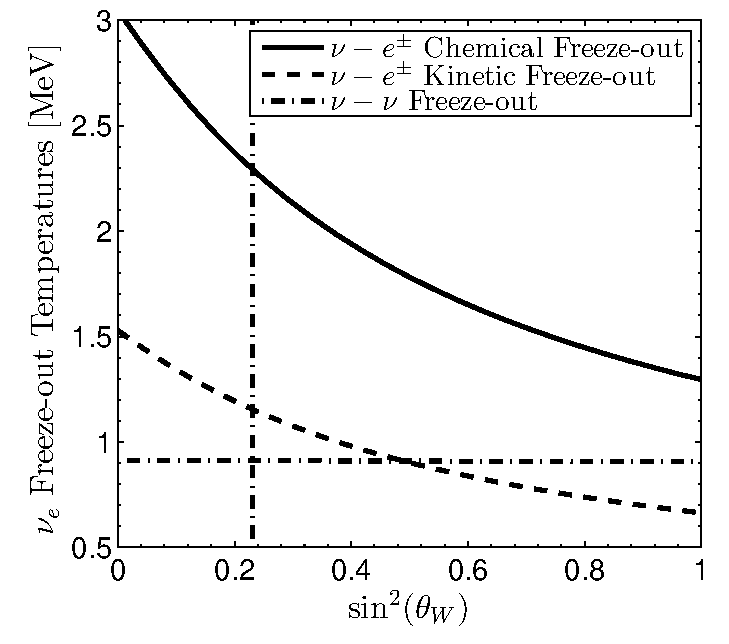
\includegraphics[width=0.47\columnwidth]{./plots/nu_e_freezeout.pdf}
\hspace{1mm}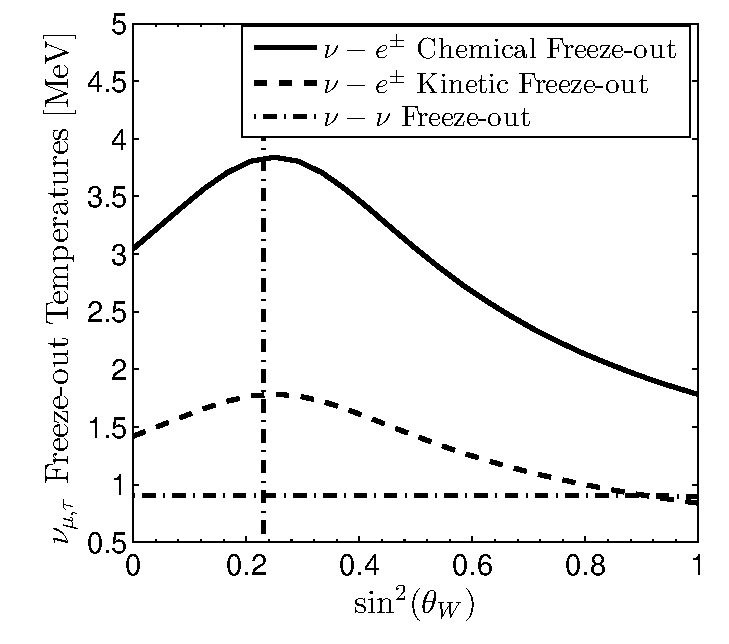
\includegraphics[width=0.47\columnwidth]{./plots/nu_mu_freezeout.pdf}}
\centerline{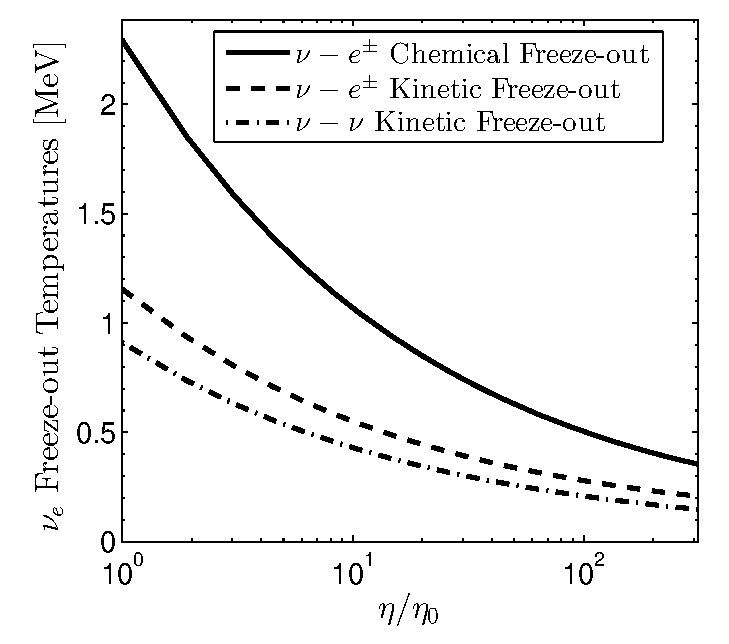
\includegraphics[width=0.47\columnwidth]{./plots/nu_e_freezeout_GF.pdf}
\hspace{1mm}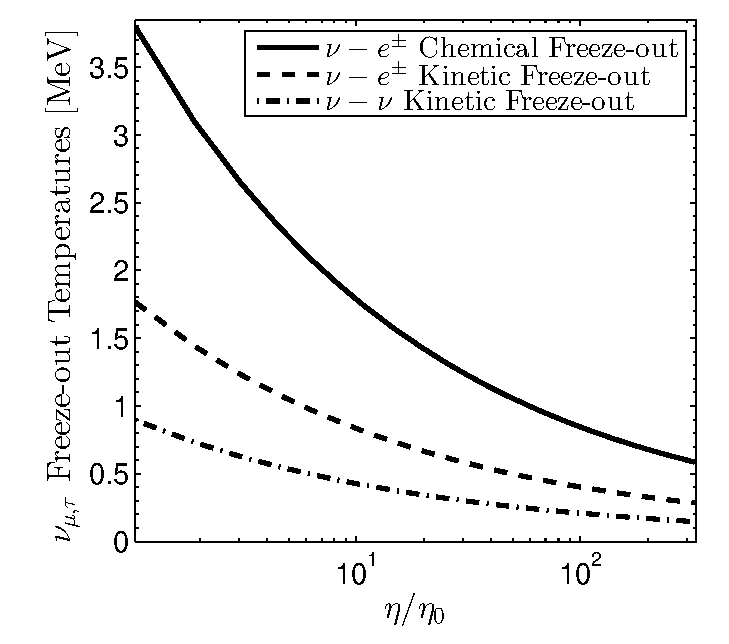
\includegraphics[width=0.47\columnwidth]{./plots/nu_mu_freezeout_GF.pdf}}
\caption{Freeze-out temperatures for electron neutrinos (left) and $\mu$, $\tau$ neutrinos (right) for the three types of freeze-out processes adapted from paper [\cite{Birrell:2014uka}]. Top panels print temperature curves as a function of $\sin^2\theta_W$ for $\eta=\eta_0$, the vertical dashed line is $\sin^2\theta_W=0.23$; bottom panels are printed as a function of relative change in interaction strength $\eta/\eta_0$ obtained for $\sin^2\theta_W=0.23$.}
\label{fig:freezeoutT}
 \end{figure}
%~~~~~~~~~~~~~~~~~~~~~~~~~~~~~~~~~~~~~~~~~~~~~
\clearpage



%%%%%%%%%%%%%%%%%%%
\subsection{Lepton number and effective number of neutrinos}

Neutrinos decoupled from the cosmic plasma in the early Universe at a temperature of $T=\mathcal{O}(2\mathrm{MeV})$ and became free-streaming. However, after freezeout neutrinos still continue to play a significant role in the evolution of the Universe and have a huge impact on cosmological observations such as Big Bang Nucleosynthesis (BBN), the Cosmic Microwave Background (CMB), and the matter spectrum for large scale structure. This is due to the sensitivity of the Hubble parameter to the total energy density in the Universe. Besides photons, neutrinos are the most abundant species and contribute significantly to the relativistic energy density throughout the early Universe, affecting the Hubble expansion rate significantly. 

The contribution of energy density from the neutrino sector can be described by the effective number of neutrinos $N_{\nu}^{\mathrm{eff}}$, which captures the number of relativistic degrees of freedom for neutrinos as well as any reheating that occurred in the sector after freeze-out. The effective number of neutrino is defined as 
\begin{align}\label{Neff}
N_\nu^{\mathrm{eff}}\equiv\frac{\rho^{\mathrm{tot}}_\nu}{\frac{7\pi^2}{120}\left(\frac{4}{11}\right)^{4/3}T_\gamma^4}\;,
\end{align}
where $\rho_\nu^{\mathrm{tot}}$ is the total energy density in neutrinos and $T_\gamma$ is the photon temperature. $N_\nu^{\mathrm{eff}}$ is defined such that three neutrino flavors with zero participation of neutrinos in reheating during $e^\pm$ annihilation results in $N_\nu^{\mathrm{eff}}=3$. The factor of $\left(4/11\right)^{1/3}$ relates the photon temperature to the free-streaming neutrinos temperature, under the assumption of zero neutrino reheating after $e^\pm$ annihilation. The currently accepted theoretical value is $N_\nu^{\mathrm{eff}}=3.046$, after including the slight effect of neutrino reheating [\cite{Mangano:2005cc,Birrell:2014uka}]. The favored value of $N_\nu^{\mathrm{eff}}$ can be found by fitting to CMB data. In 2013 the Planck collaboration found $N_\nu^{\mathrm{eff}}=3.36\pm0.34$ (CMB only) and $N_\nu^{\mathrm{eff}}= 3.62\pm0.25$ (CMB and $H_0$)~[\cite{Planck:2013pxb}].

To explain the experimental value of $N_\nu^{\mathrm{eff}}$, many studies aim to improve the calculation of neutrino decoupling in the early Universe, including exploring the dependence of freeze-out on natural constants~[\cite{Birrell:2014uka}], the entropy transfer from $e^\pm$ annihilation and finite temperature correction~[\cite{Dicus:1982bz,Heckler:1994tv,Fornengo:1997wa}], neutrino decoupling with flavor oscillations~[\cite{Mangano:2001iu,Mangano:2005cc}], and investigating nonstandard neutrino interactions [\cite{Morgan:1981zy,Fukugita:1987uy,Elmfors:1997tt,Vogel:1989iv,Mangano:2006ar,Giunti:2008ve,Mangano:2006ar}].% However, the effective number of neutrino $N_\nu^{\mathrm{eff}}$ can be a consequence of fundamental physics principle.


The standard cosmological model assumes that the lepton asymmetry $L\equiv  [N_\mathrm{L}-N_{\overline{\mathrm{L}}}] /N_\gamma $  (normalized with the photon number) 
between leptons and anti-leptons is small, similar to the baryon asymmetry $B=[N_\mathrm{B}-N_{\overline{\mathrm{B}}}]/N_\gamma $; most often it is assumed $L=B$. Barenboim, Kinney, and Park~[\cite{Barenboim:2016shh,Barenboim:2017dfq}] noted that the lepton asymmetry of the Universe is one of the most weakly constrained parameters is cosmology and they propose that models with leptogenesis are able to accommodate a large lepton number asymmetry surviving up to today.  Moreover, the discrepancy between $H_\mathrm{CMB}$ and $H_0$ has increased~[\cite{riess2018new,Riess:2018byc,Planck:2018vyg}]. The Hubble tension and the possibility that leptogenesis in the early Universe resulted in neutrino asymmetry motivate our study of the dependence of $N_\nu^{\mathrm{eff}}$ on lepton asymmetry, $L$. In our work~[\cite{Yang:2018oqg}] we consider $L\simeq 1$ and explore how this large cosmological lepton yield relates to the effective number of (Dirac) neutrinos $N^{\mathrm{eff}}_\nu$. 

\subsubsection{Relation between $N_\nu^{\mathrm{eff}}$ and neutrino chemical potential}
We consider now neutrinos decouple~[\cite{Birrell:2014gea}] at a temperature of $T_f\simeq 2\,\mathrm{MeV}$ and are subsequently free-streaming. Assuming exact thermal equilibrium at the time of decoupling, the neutrino distribution can be subsequently written as (see~[\cite{Birrell:2012gg}] and references therein)
\begin{align}
\label{fnudef}
&f_\nu=\frac{1}{\exp{\left(\sqrt{\frac{E^2-m_\nu^2}{T_\nu^2}+\frac{m^2_\nu}{T^2_f}}-\sigma\frac{\mu_\nu}{T_f}\right)+1}}\;,\qquad T_\nu\equiv\frac{a(t_f)}{a(t)}T_f,
\end{align}
where $\sigma=+1(-1)$ denotes particles (antiparticles) and we define the effective neutrino temperature $T_\nu$  by the red-shifting of momentum in the comoving volume element of the Universe.

Since the freeze-out temperature $T_f\gg m_\nu$ and also neutrino temperature $T_\nu\gg m_\nu$ in the domain of our analysis, we consider the massless limit in Eq.\;(\ref{fnudef}). Under this approximation, the total neutrino energy density can be written as
\begin{align}
\label{Energy_Density}
\rho_\nu^{\mathrm{tot}}
&=\frac{g_\nu\,T_\nu^4}{2\pi^2}\left[\frac{7\pi^4}{60}+\frac{\pi^2}{2}\left(\frac{\mu_\nu}{T_f}\right)^{\!\!2}+\frac{1}{4}\left(\frac{\mu_\nu}{T_f}\right)^{\!\!4}\right].
\end{align}
Substituting Eq.\;(\ref{Energy_Density}) into the definition of the effective number of neutrinos Eq.~(\ref{Neff}), we obtain 
\begin{align}
\label{Neff_002}
N_\nu^{\mathrm{eff}}\!\!
=\!3\!\left(\frac{11}{4}\right)^{\!\!\frac{4}{3}}\!\!\left(\frac{T_\nu}{T_\gamma}\right)^{\!\!4}\!
\left[1\!+\!\frac{30}{7\pi^2}\!\!\left(\frac{\mu_\nu}{T_f}\right)^{\!\!2} 
\!\!+\frac{15}{7\pi^4}\!\!\left(\frac{\mu_\nu}{T_f}\right)^{\!\!4}\right].
\end{align}
From Eq.\;(\ref{Neff_002}) we have for the standard photon reheating ratio $T_\nu/T_\gamma=(4/11)^{1/3}$ [\cite{Kolb:1990vq}] and degeneracy $g_\nu=3$ (flavor), the relation between the effective number of neutrinos and the chemical potential at freezeout
\begin{align}
\label{Neff_Potential}
N_\nu^{\mathrm{eff}}=3\left[1+\frac{30}{7\pi^2}\left(\frac{\mu_\nu}{T_f}\right)^{\!\!2}+ \frac{15}{7\pi^4} \left(\frac{\mu_\nu}{T_f}\right)^{\!\!4}\right].
\end{align}
To solve the neutrino chemical potential $\mu_\nu/T_f$ as a function of the effective number of neutrinos, we can neglect the $(\mu_\nu/T_f)^4$ term in Eq.\;(\ref{Neff_Potential}) because $m_\nu\ll T_f$ and obtain
\begin{align}\label{Solution}
\frac{\mu_\nu}{T_f}=\pm\sqrt{\frac{7\pi^2}{30}\left(\frac{N_\nu^{\mathrm{eff}}}{3}-1\right)}.
%=&\pm \pi\sqrt{\sqrt{1+\frac{7}{15}\left(\frac{N_\nu^{\mathrm{eff}}}{3}-1\right)}-1}%\approx
\end{align}
In Fig.\;\ref{Chemical_Potential_Neff} we plot the free-streaming neutrino chemical potential $|\mu_\nu|/T_f$ as a function of the effective number of neutrinos $N_\nu^{\mathrm{eff}}$. For comparison, the solid (blue) line is the exact solution of $|\mu_\nu|/T_f$ by solving Eq.~(\ref{{Neff_Potential}}) numerically, and the (red) dashed line is the approximate solution Eq.~(\ref{Solution}) by neglecting the $(\mu_\nu/T_f)^4$ in calculation. In the parameter range of interest, we show that the term $(\mu_\nu/T_f)^4$ only contributes $\approx 2\%$ to the calculation and henceforth we neglect it, and use the approximation Eq.\;(\ref{Solution}). 

The SM value of the effective number of neutrinos, $N_\nu^{\mathrm{eff}}=3$, is obtained under the assumption that the neutrino chemical potentials are not essential, {\it i.e.\/}, $\mu_\nu\ll T_f$. From Fig.\;\ref{Chemical_Potential_Neff}, to interpret the literature values $N_\nu^{\mathrm{eff}}=3.36\pm0.34$ (CMB only) and $N_\nu^{\mathrm{eff}}= 3.62\pm0.25$ (CMB and $H_0$), we require $0.52\leqslant\mu_\nu/T_f\leqslant0.69$. These values suggest  a possible neutrino-antineutrino asymmetry at freezeout, {\it i.e.\/} a difference between the number densities of neutrinos and antineutrinos.
%%%%%%%%%%%%%%%%%%%%%%%%%%%%%%%%%%%%%%%%%%%%%%%%%%%%%%%%%%%%%%%%%%
\begin{figure}[t]
\begin{center}
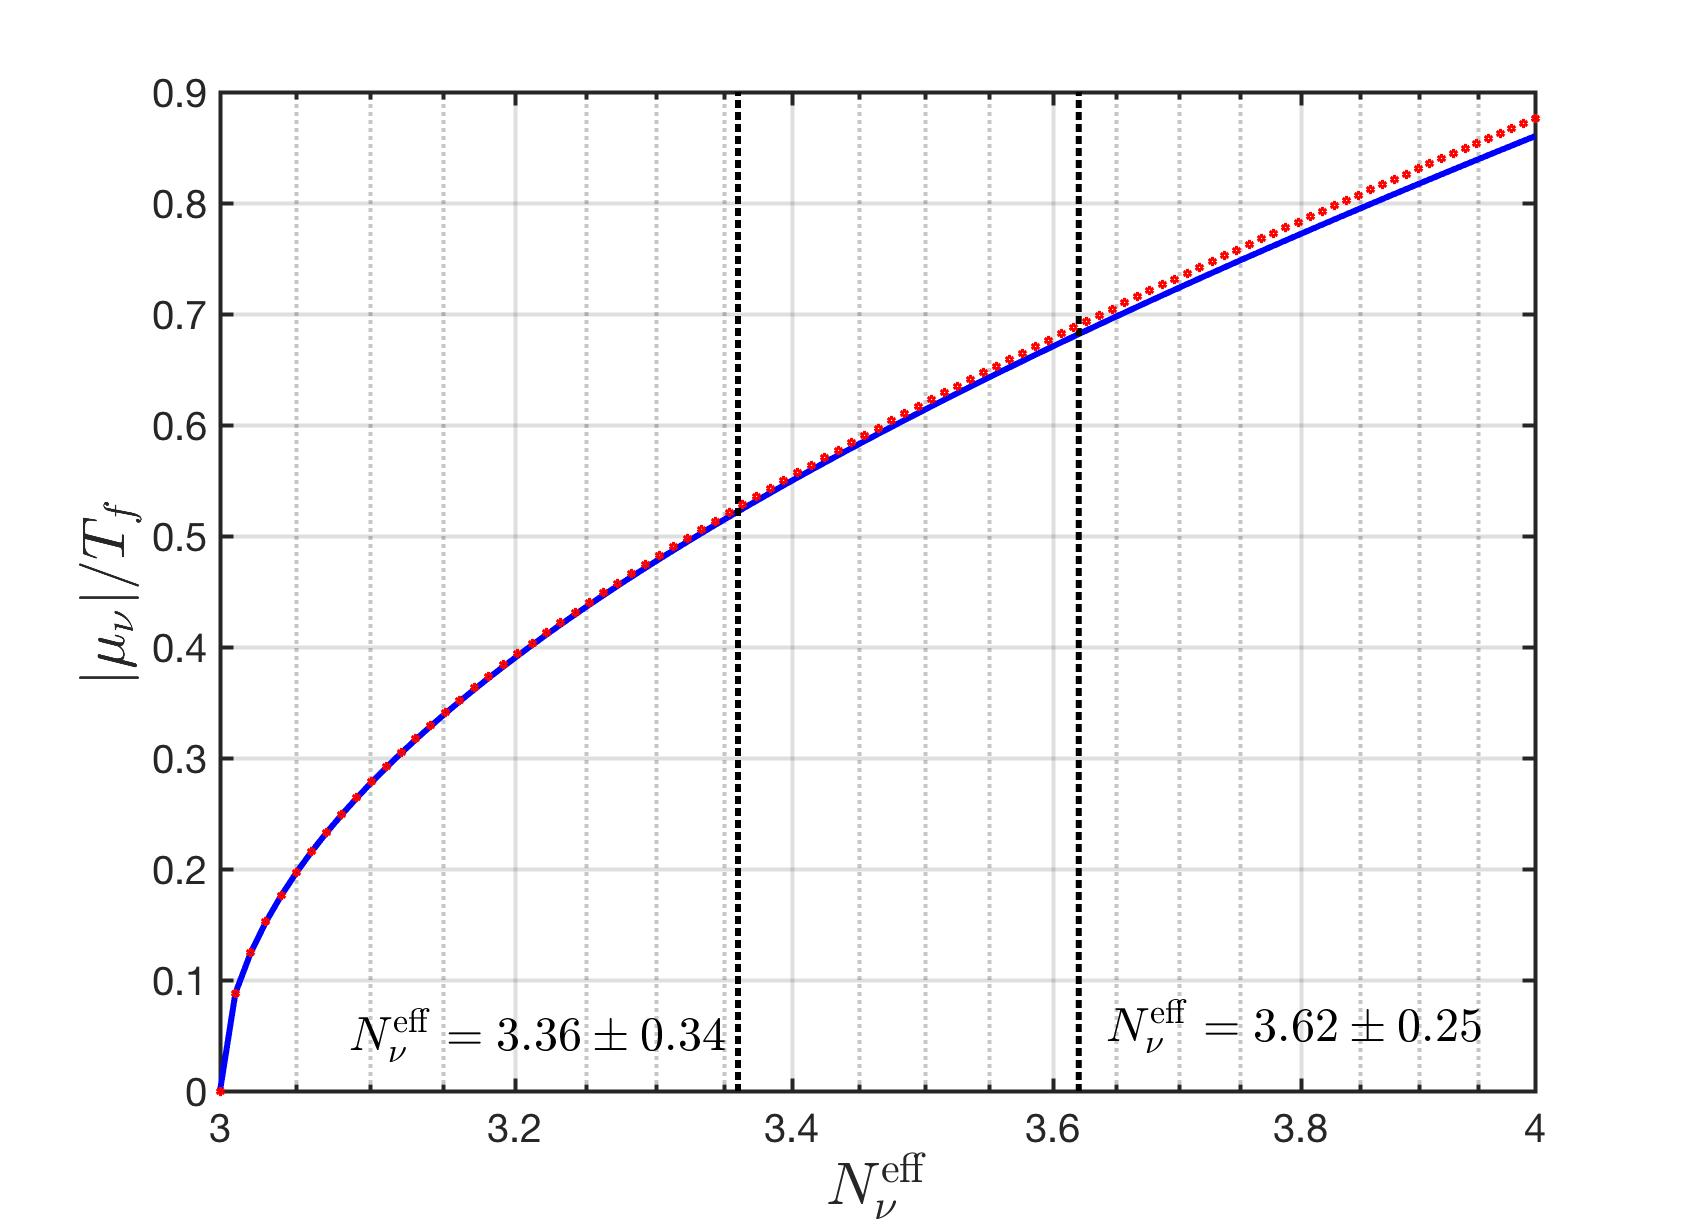
\includegraphics[width=\textwidth]{./plots/Chemical_Potential_Neff}
\caption{The free-streaming neutrino chemical potential $|\mu_\nu|/T_f$ as a function of the effective number of neutrinos $N_\nu^{\mathrm{eff}}$. The solid (blue) line is the exact solution and the (red) dashed line is the approximate solution neglecting the $(\mu_\nu/T_f)^4$ term; the maximum difference in the domain shown is about $2\%$.}
\label{Chemical_Potential_Neff}
\end{center}
\end{figure}
%%%%%%%%%%%%%%%%%%%%%%%%%%%%%%%%%%%%%%%%%%%%%%%%%%%%%%%%%%%%%%%%%%%



\subsubsection{Dependence of $N_\nu^{\mathrm{eff}}$ on lepton asymmetry}
We now obtain the relation between neutrino chemical potential and the baryon to lepton ratio. Let us consider the neutrino freezeout temperature $T_f\simeq 2.0$ MeV; here we treat neutrino freezeout as occurring instantaneously and prior to $e^\pm$ annihilation (implying zero neutrino reheating). Comoving lepton (and baryon) number is conserved after the epoch of leptogenesis (baryogenesis, respectively) which precedes the epoch  under consideration in this work ($T\lesssim 2$\;MeV). %However, the photon number $N_\gamma$ changes due to reheating, and accommodates the large number of photons originating from $e^+e^-$-annihilation.% We present results in terms of the current epoch photon number. 

The lepton-density asymmetry $\ell $ at neutrino freeze-out can be written as
\begin{align}
\ell_f \equiv\big(n_e-n_{\overline{e}}\big)_f+\sum_{i=e,\mu, \tau}\big(n_{\nu_i}-n_{\overline{\nu}_i}\big)_f,
\end{align}
where we use the subscript $f$ to indicate that the quantities should be evaluated at the neutrino freeze-out temperature. As a first approximation, here we assume that all neutrinos freeze-out at the same temperature and their chemical potentials are the same; {\it i.e.\/},
\begin{align}
\mu_\nu=\mu_{\nu_e}=\mu_{\nu_\mu}=\mu_{\nu_\tau}.
\end{align}
Furthermore, neutrino oscillation implies that neutrino number is freely exchanged between flavors; {\it i.e.\/}, $\nu_e\rightleftharpoons\nu_\mu\rightleftharpoons\nu_\tau$, and we can assume that all neutrino flavors share the same population. Under these assumptions, the lepton-density asymmetry can be written as
\begin{align}
\label{L_asymmetry} 
\ell_f=\big(n_e-n_{\overline{e}}\big)_f+\big(n_{\nu}-n_{\overline{\nu}}\big)_f,
\end{align}
where the three flavors are accounted for by taking the degeneracy $g_\nu=3$ in the last term. The difference in yield of neutrinos and antineutrinos can be written as
\begin{align}
\label{Excess_Neutrino}
\left(n_\nu-n_{\overline{\nu}}\right)_f=\frac{g_\nu}{6\pi^2}T^3_f\bigg[\pi^2\left(\frac{\mu_\nu}{T_f}\right)+\left(\frac{\mu_\nu}{T_f}\right)^{\!\!3}\bigg].
\end{align}


On the other hand, the baryon-density asymmetry $b$ at neutrino freezeout is given by
\begin{align}
\label{B_asymmetry}
b_f \equiv\big(n_p-n_{\overline{p}}\big)_f+\big(n_n-n_{\overline{n}}\big)_f \approx \big(n_p+n_n\big)_f,
\end{align}
where $n_{\overline{n}}$ and $n_{\overline{p}}$ are negligible in the temperature range we consider here. Taking the ratio $\ell_f/b_f$, using charge neutrality, and introducing the entropy density we obtain
\begin{align}\label{Lf_Bf}
\left(\frac{\ell_f}{b_f}\right)  
\approx\left(\frac{n_p}{n_B} \right)_f+\left(n_{\nu}-n_{\overline{\nu}}\right)_f \left(\frac{s}{n_B}\right)_f \frac{1}{s_f},\qquad n_B=(n_p+n_n),
\end{align}
where we introduce the notation $n_B$ for the baryon number density. The proton concentration at neutrino freeze-out is given by
\begin{align}
\label{X_proton}
\left(\frac{n_p}{n_B}\right)_f&=\frac{1}{1+(n_n/n_p)_f}=\frac{1}{1+\exp{\big[-\left(Q+\mu_\nu\right)/T_f\big]}},
\end{align}
with $Q=m_n-m_p=1.293\,\mathrm{MeV}$. We neglect the electron chemical potential in the last step because the $e^\pm$ asymmetry is determined by the proton density, and at energies of order a few MeV, the proton density is small, {\it i.e.\/}, $\mu_e\ll T_f$. 

However, as we will see, for our study of $N_\nu^{\mathrm{eff}}$ we will be interested in the case of a large lepton-to-baryon ratio. From Eq.\;(\ref{X_proton}) it is apparent that this can only be achieved through the second term in Eq.\;(\ref{Lf_Bf}), with the first term then being negligible, as it is smaller than $1$. So we further approximate
\begin{align}\label{L_B_ratio}
\left(\frac{\ell_f}{b_f}\right)  
\approx\left(n_{\nu}-n_{\overline{\nu}}\right)_f \left(\frac{s}{n_B}\right)_f \frac{1}{s_f}.
\end{align}
We retained the full expression Eq.\;(\ref{X_proton}) in our above discussion to show that the presence of a chemical potential $\mu_\nu\simeq 0.2\,Q$ could lead to small, perhaps noticeable, effects on pre-BBN proton and neutron abundance. We defer this unrelated discussion to a separate future work. Note that for large $|\mu_\nu|$, Eq.\;(\ref{L_B_ratio}) implies that the signs of $\mu_\nu$ and $\ell_f$ are the same. However, for very small $\mu_\nu$ the sign of $\ell_f$ is determined by the interplay between (anti)electrons and (anti)neutrinos; {\it i.e.\/}, there is competition between the two terms in Eq.\;(\ref{L_asymmetry}).

In general, the total entropy density at freeze-out can be written
\begin{align}
\label{Entropy_density}
s_f=\frac{2\pi^2}{45}g^s_\ast(T_f)\,T_f^3,
\end{align}
where the $g^s_\ast$ counts the degree of freedom for relativistic particles~[\cite{Kolb:1990vq}]. At $T_f\simeq 2\mathrm{MeV}$, the relativistic species in the early Universe are photons, electron/positrons, and $3$ neutrino species. We have
\begin{align}
g^s_{\ast}&= g_\gamma+\frac{7}{8}\,g_{e^\pm}+\frac{7}{8}\,g_{\nu\bar{\nu}}\left(\frac{T_\nu}{T_\gamma}\right)^{\!\!3}\bigg[1+\frac{15}{7\pi^2}\left(\frac{\mu_\nu}{T_f}\right)^{\!\!2}\bigg]=10.75+\frac{45}{4\pi^2}\left(\frac{\mu_\nu}{T_f}\right)^{\!\!2}\;,
\end{align}
where the degrees of freedom are given by $g_\gamma=2$, $g_{e^\pm}=4$, and $g_{\nu\bar{\nu}}=6$, and we have $T_\nu=T_\gamma=T_f$ at neutrino freeze-out.

%%%%%%%%%%%%%%%%%%%%%%%%%%%%%%%%%
\begin{figure}[h]
\begin{center}
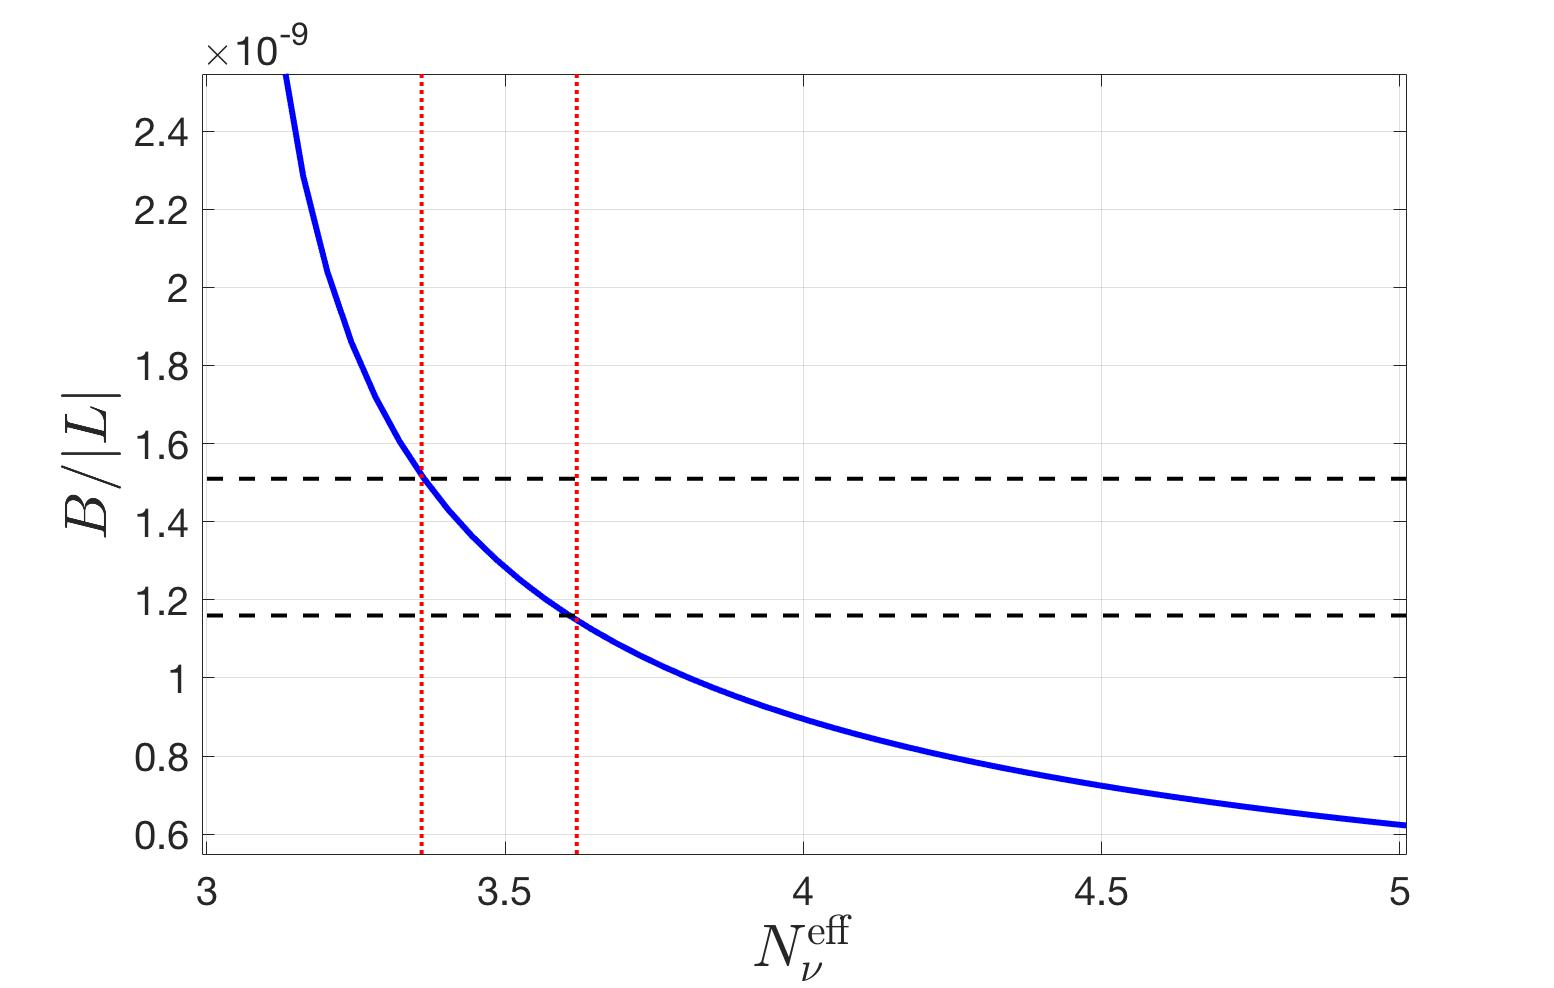
\includegraphics[width=\textwidth]{./plots/Ratio_BL}
\caption{The ratio $B/|L|$ between the net baryon number and the net lepton number as a function of $N^{\mathrm{eff}}_\nu$: The solid blue line shows $B/|L|$. The vertical (red) dotted lines represent the values $3.36\leqslant N_\nu^{\mathrm{eff}}\leqslant3.62$, which correspond to $1.16 \times 10^{-9}\leqslant B/|L|\leqslant 1.51 \times 10^{-9}$ (horizontal dashed lines).}
\label{BL_Ratio}
\end{center}
\end{figure}
%%%%%%%%%%%%%%%%%%%%%%%%%%%%%%%%%%%%%%%%%%%%%%%%%%%%%%%%%%%%%%%%%%

Finally, since the entropy-per-baryon from neutrino freeze-out up to the present epoch is constant, we can obtain this value by considering the Universe's entropy content today~[\cite{Fromerth:2012fe}]. For $T\ll1\,\mathrm{MeV}$, the entropy content today is carried by photons and neutrinos, yielding
\begin{align}
\label{Nb_S}
\left(\frac{s}{n_B}\right)_{t_0}&=\frac{\sum_i\,s_i}{n_B}=\frac{n_\gamma}{n_B}\,\bigg(\frac{s_\gamma}{n_\gamma}+\frac{s_\nu}{n_\gamma}+\frac{s_{\bar{\nu}}}{n_\gamma}\bigg)\;\\
&=\left(\frac{1}{B}\right)_{\!\!t_0}\!\!\left[\frac{s_\gamma}{n_\gamma}+\frac{4}{3T_\nu}\frac{\rho_\nu^{\mathrm{tot}}}{n_\gamma}-\frac{\mu_\nu}{T_f}\left(\frac{n_\nu-n_{\bar{\nu}}}{n_\gamma}\right)\right]_{t_0}\;,
\end{align}
where $t_0$ denotes the present day values, we have $B=n_B/n_\gamma= 0.605\times10^{-9}$ (CMB)~[\cite{ParticleDataGroup:2016lqr}] from today's observation. The entropy per particle for a massless boson at zero chemical potential is $(s/n)_{\mathrm{boson}}\approx 3.602$.

Substituting Eq.\;(\ref{Excess_Neutrino}) and Eq.\;(\ref{Entropy_density}) into Eq.\;(\ref{L_B_ratio}) yields the lepton-to-baryon ratio
\begin{align}\label{L_B_ratio_final}
&\frac{L}{B}=\frac{45}{4\pi^4}\frac{\pi^2(\mu_\nu/T_f)+(\mu_\nu/T_f)^3}{10.75+{45}(\mu_\nu/T_f)^2/{4\pi^2}}\left(\frac{s}{n_B}\right)_{\!\!t_0}\;,
\end{align}
in terms of $\mu_\nu/T_f$ which is given by Eq.(\ref{Solution}) and the present day entropy-per-baryon ratio. In Fig.\;\ref{BL_Ratio} we show the ratio between the net baryon number and the net lepton number as a function of the effective number of neutrino species $N^{\mathrm{eff}}_\nu$ with the parameter $ B|_{t_0} =0.605\times 10^{-9}$(CMB). We find that the values $N_\nu^{\mathrm{eff}}=3.36\pm0.34$ and $N_\nu^{\mathrm{eff}}= 3.62\pm0.25$ require the ratio between baryon number and lepton number to be $1.16 \times 10^{-9} \leqslant\, B/|L| \leqslant 1.51\times 10^{-9}$. These values are close to the baryon-to-photon ratio $0.57 \times 10^{-9} \leqslant B  \leqslant 0.67\times 10^{-9}$. 


In summary, motivated by the necessity to explain a slightly faster Universe expansion, we believe that there is need for additional unobserved particles,  leading to an increase  in the Universe expansion rate. Considerable effort has been made in this direction, e.g., by introducing exotic and new \lq dark\rq\ particles, see~[\cite{Birrell:2014cja}] and references therein. In this work a similar effect is achieved by introducing lepton asymmetry in the Universe. We connected the lepton asymmetry in the Universe with the chemical neutrino potential $\mu_\nu$,
and further evaluated the consequences for the Universe expansion. We have explored the other natural scenario regarding the baryon number-to-lepton number ratio. Instead of $B\simeq |L|$, we found that $0.4\leqslant|L| \leqslant0.52$ and $B\simeq 1.33\times 10^{-9}|L|$ reconciles the CMB and current epoch results for the Hubble expansion parameter.
%The standard cosmological model assumes (arbitrarily) that the asymmetry between leptons and anti-leptons is small, similar to the baryon asymmetry; most often it is assumed $L=B$. We consider $L\simeq 1$ and explore how this large cosmological lepton yield relates to the effective number of (Dirac) neutrinos $N^{\mathrm{eff}}_\nu$.  we have explored the other natural scenario regarding the baryon number-to-lepton number ratio. Instead of $B\simeq |L|$, we found that $0.4\leqslant|L| \leqslant0.52$ and $B\simeq 1.33\times 10^{-9}|L|$ reconciles the CMB and current epoch results for the Hubble expansion parameter.

The large lepton asymmetry from cosmic neutrino can also affect the neutron lifespan in cosmic plasma which is one of the important parameter controlling BBN element abundances. 
In general the neutron lifespan dependence on temperature of the cosmic medium. When temperature $T=\mathcal{O}(\mathrm{MeV})$, neutron decay occurs in the plasma of electron/positron and 
 neutrino/antineutrino. Electrons and neutrinos in the background plasma can reduce the neutron decay rate by Fermi suppression to the neutron decay rate. Furthermore, the neutrino background can still provide the suppression after electron/positron pair annihilation becomes nearly complete. In this case,the large neutrino chemical potential from lepton asymmetry would play an important role and needs to be accounted for in the precision study of the neutron lifespan in the cosmic plasma.